%%%%%%%%%%%%%%%%%%%%%%%%%%%%%%%%%%%%%%%%%
% Lachaise Assignment
% LaTeX Template
% Version 1.0 (26/6/2018)
%
% This template originates from:
% http://www.LaTeXTemplates.com
%
% Authors:
% Marion Lachaise & François Févotte
% Vel (vel@LaTeXTemplates.com)
%
% License:
% CC BY-NC-SA 3.0 (http://creativecommons.org/licenses/by-nc-sa/3.0/)
%
%%%%%%%%%%%%%%%%%%%%%%%%%%%%%%%%%%%%%%%%%

%----------------------------------------------------------------------------------------
%	PACKAGES AND OTHER DOCUMENT CONFIGURATIONS
%----------------------------------------------------------------------------------------

\documentclass{article}

%%%%%%%%%%%%%%%%%%%%%%%%%%%%%%%%%%%%%%%%%
% Lachaise Assignment
% Structure Specification File
% Version 1.0 (26/6/2018)
%
% This template originates from:
% http://www.LaTeXTemplates.com
%
% Authors:
% Marion Lachaise & François Févotte
% Vel (vel@LaTeXTemplates.com)
%
% License:
% CC BY-NC-SA 3.0 (http://creativecommons.org/licenses/by-nc-sa/3.0/)
%
%%%%%%%%%%%%%%%%%%%%%%%%%%%%%%%%%%%%%%%%%

%----------------------------------------------------------------------------------------
%	PACKAGES AND OTHER DOCUMENT CONFIGURATIONS
%----------------------------------------------------------------------------------------

\usepackage{amsmath,amsfonts,stmaryrd,amssymb} % Math packages

\usepackage{enumerate} % Custom item numbers for enumerations

\usepackage[ruled]{algorithm2e} % Algorithms

\usepackage[framemethod=tikz]{mdframed} % Allows defining custom boxed/framed environments

\usepackage{listings} % File listings, with syntax highlighting

\usepackage{color} %red, green, blue, yellow, cyan, magenta, black, white
\definecolor{mygreen}{RGB}{28,172,0} % color values Red, Green, Blue
\definecolor{mylilas}{RGB}{170,55,241}
\usepackage{float}
\usepackage{amsmath}% http://ctan.org/pkg/amsmath
\newcommand\Inn{%
  \mathrel{\ooalign{$\subset$\cr\hfil\scalebox{0.8}[1]{$=$}\hfil\cr}}%
}
% \mathcode`*=\string"8000

\lstset{
	basicstyle=\ttfamily, % Typeset listings in monospace font
}


% matlab desciption
% usage \lstinputlisting{/path/to/matlab/code.m}

\lstset{language=Matlab,%
    %basicstyle=\color{red},
    breaklines=true,%
    morekeywords={matlab2tikz},
    keywordstyle=\color{blue},%
    morekeywords=[2]{1}, keywordstyle=[2]{\color{black}},
    identifierstyle=\color{black},%
    stringstyle=\color{mylilas},
    commentstyle=\color{mygreen},%
    showstringspaces=false,%without this there will be a symbol in the places where there is a space
    numbers=none,%
    numberstyle={\tiny \color{black}},% size of the numbers
    numbersep=9pt, % this defines how far the numbers are from the text
    emph=[1]{for,end,break},emphstyle=[1]\color{red}, %some words to emphasise
    %emph=[2]{word1,word2}, emphstyle=[2]{style},
}


%----------------------------------------------------------------------------------------
%	DOCUMENT MARGINS
%----------------------------------------------------------------------------------------

\usepackage{geometry} % Required for adjusting page dimensions and margins

\geometry{
	paper=a4paper, % Paper size, change to letterpaper for US letter size
	top=2.5cm, % Top margin
	bottom=3cm, % Bottom margin
	left=2.5cm, % Left margin
	right=2.5cm, % Right margin
	headheight=14pt, % Header height
	footskip=1.5cm, % Space from the bottom margin to the baseline of the footer
	headsep=1.2cm, % Space from the top margin to the baseline of the header
	%showframe, % Uncomment to show how the type block is set on the page
}

%----------------------------------------------------------------------------------------
%	FONTS
%----------------------------------------------------------------------------------------

\usepackage[utf8]{inputenc} % Required for inputting international characters
\usepackage[T1]{fontenc} % Output font encoding for international characters

\usepackage{XCharter} % Use the XCharter fonts

%----------------------------------------------------------------------------------------
%	COMMAND LINE ENVIRONMENT
%----------------------------------------------------------------------------------------

% Usage:
% \begin{commandline}
%	\begin{verbatim}
%		$ ls
%
%		Applications	Desktop	...
%	\end{verbatim}
% \end{commandline}

\mdfdefinestyle{commandline}{
	leftmargin=10pt,
	rightmargin=10pt,
	innerleftmargin=15pt,
	middlelinecolor=black!50!white,
	middlelinewidth=2pt,
	frametitlerule=false,
	backgroundcolor=black!5!white,
	frametitle={Command Line},
	frametitlefont={\normalfont\sffamily\color{white}\hspace{-1em}},
	frametitlebackgroundcolor=black!50!white,
	nobreak,
}

% Define a custom environment for command-line snapshots
\newenvironment{commandline}{
	\medskip
	\begin{mdframed}[style=commandline]
}{
	\end{mdframed}
	\medskip
}

%----------------------------------------------------------------------------------------
%	FILE CONTENTS ENVIRONMENT
%----------------------------------------------------------------------------------------

% Usage:
% \begin{file}[optional filename, defaults to "File"]
%	File contents, for example, with a listings environment
% \end{file}

\mdfdefinestyle{file}{
	innertopmargin=1.6\baselineskip,
	innerbottommargin=0.8\baselineskip,
	topline=false, bottomline=false,
	leftline=false, rightline=false,
	leftmargin=2cm,
	rightmargin=2cm,
	singleextra={%
		\draw[fill=black!10!white](P)++(0,-1.2em)rectangle(P-|O);
		\node[anchor=north west]
		at(P-|O){\ttfamily\mdfilename};
		%
		\def\l{3em}
		\draw(O-|P)++(-\l,0)--++(\l,\l)--(P)--(P-|O)--(O)--cycle;
		\draw(O-|P)++(-\l,0)--++(0,\l)--++(\l,0);
	},
	nobreak,
}

% Define a custom environment for file contents
\newenvironment{file}[1][File]{ % Set the default filename to "File"
	\medskip
	\newcommand{\mdfilename}{#1}
	\begin{mdframed}[style=file]
}{
	\end{mdframed}
	\medskip
}

%----------------------------------------------------------------------------------------
%	NUMBERED QUESTIONS ENVIRONMENT
%----------------------------------------------------------------------------------------

% Usage:
% \begin{question}[optional title]
%	Question contents
% \end{question}

\mdfdefinestyle{question}{
	innertopmargin=1.2\baselineskip,
	innerbottommargin=0.8\baselineskip,
	roundcorner=5pt,
	nobreak,
	singleextra={%
		\draw(P-|O)node[xshift=1em,anchor=west,fill=white,draw,rounded corners=5pt]{%
		Question \theQuestion\questionTitle};
	},
}

\newcounter{Question} % Stores the current question number that gets iterated with each new question

% Define a custom environment for numbered questions
\newenvironment{question}[1][\unskip]{
	\bigskip
	\stepcounter{Question}
	\newcommand{\questionTitle}{~#1}
	\begin{mdframed}[style=question]
}{
	\end{mdframed}
	\medskip
}

%----------------------------------------------------------------------------------------
%	WARNING TEXT ENVIRONMENT
%----------------------------------------------------------------------------------------

% Usage:
% \begin{warn}[optional title, defaults to "Warning:"]
%	Contents
% \end{warn}

\mdfdefinestyle{warning}{
	topline=false, bottomline=false,
	leftline=false, rightline=false,
	nobreak,
	singleextra={%
		\draw(P-|O)++(-0.5em,0)node(tmp1){};
		\draw(P-|O)++(0.5em,0)node(tmp2){};
		\fill[black,rotate around={45:(P-|O)}](tmp1)rectangle(tmp2);
		\node at(P-|O){\color{white}\scriptsize\bf !};
		\draw[very thick](P-|O)++(0,-1em)--(O);%--(O-|P);
	}
}

% Define a custom environment for warning text
\newenvironment{warn}[1][Warning:]{ % Set the default warning to "Warning:"
	\medskip
	\begin{mdframed}[style=warning]
		\noindent{\textbf{#1}}
}{
	\end{mdframed}
}

%----------------------------------------------------------------------------------------
%	INFORMATION ENVIRONMENT
%----------------------------------------------------------------------------------------

% Usage:
% \begin{info}[optional title, defaults to "Info:"]
% 	contents
% 	\end{info}

\mdfdefinestyle{info}{%
	topline=false, bottomline=false,
	leftline=false, rightline=false,
	nobreak,
	singleextra={%
		\fill[black](P-|O)circle[radius=0.4em];
		\node at(P-|O){\color{white}\scriptsize\bf i};
		\draw[very thick](P-|O)++(0,-0.8em)--(O);%--(O-|P);
	}
}

% Define a custom environment for information
\newenvironment{info}[1][Info:]{ % Set the default title to "Info:"
	\medskip
	\begin{mdframed}[style=info]
		\noindent{\textbf{#1}}
}{
	\end{mdframed}
}
 % Include the file specifying the document structure and custom commands
\usepackage{graphicx}
\newcommand{\ts}{\textsuperscript}
<<<<<<< HEAD
\usepackage{float}

=======
>>>>>>> 31adf8bead0ca3f0783d74f4a70004e23d603956

%----------------------------------------------------------------------------------------
%	ASSIGNMENT INFORMATION
%----------------------------------------------------------------------------------------

\title{Computational Engineering - Engr 8103 \\ Problem Set \#6} % Title of the assignment

\author{Allen Spain\\ \texttt{avs81684@uga.edu}} % Author name and email address

\date{University of Georgia --- 22 October 2019 } % University, school and/or department name(s) and a date

%----------------------------------------------------------------------------------------

\begin{document}

\maketitle % Print the title

%----------------------------------------------------------------------------------------
%	INTRODUCTION
%----------------------------------------------------------------------------------------

\section*{Problem 1} % Unnumbered section
Show that the following is another valid second order Runge-Kutta method:

\noindent
From the 2\ts{nd} order Taylor series method:

\noindent
<<<<<<< HEAD
Where:
=======
Notation:
>>>>>>> 31adf8bead0ca3f0783d74f4a70004e23d603956

\begin{align*}
	x  \rightarrow x(t) \\
	f  \rightarrow f(t,x) \\
	f_{t}  \rightarrow \frac{\partial f}{\partial t} \\
	f_{x}  \rightarrow \frac{\partial f}{\partial x}
\end{align*}
\begin{align*}
	\boxed{x(t + h) = x + hf + \frac{h^{2}}{2}(f_{t} + ff_{x})}
\end{align*}

\noindent
From the 2\ts{nd} order Runge-Kutta method:

\begin{align*}
	K_{1} = hf \\
	K_{2} = hf(t + \frac{2}{3}h, x + \dfrac{2}{3}K_{1}) = h(f +  \frac{2}{3}h(f_{t} + ff_{x})) \\
	x(t + h) = x(t) + (K_{1} + 3K_{2})/4 \\
	= x(t) + \dfrac{hf(t,x)}{4} + 3/4(h(f + \frac{2}{3}h(f_{t} + ff_{x}))) \\
	= x(t) + \dfrac{hf}{4} + \dfrac{3hf}{4} + \dfrac{h^{2}}{2}(f_{t} + ff_{x}) \\
	\boxed{x(t + h) = x(t) + hf + \frac{h^{2}}{2}(f_{t} + ff_{x})}
 \end{align*}

<<<<<<< HEAD
\section*{Problem 2}
Show that when the fourth-order Runge-Kutta method is applied to the problem $ x^{\prime} = 2x $, the formula for advancing this solution will be

\begin{align*}
	x(t + h) = \big[1 + 2h + 2h^{2} + \frac{4}{3}h^{3} + \frac{2}{3}h^{4} \big] x(t) \\
\end{align*}

From the 4\ts{th} order Runge-Kutta method:
\begin{align*}
	K_{1} = hf = 2xh \\
	K_{2} = hf(t + \frac{h}{2}, x + \frac{K_{1}}{2}) = 2xh + 2h^{2}x \\
	K_{3} = hf(t + \frac{h}{2}, x + \frac{K_{2}}{2}) = 2xh + 2xh^{2} + 2xh^{3} \\
	K_{4} = hf(t + \frac{h}{2}, x + \frac{K_{3}}{2}) = 2xh + 4xh^{2} + 4xh^{3} + 4xh^{4} \\
	x(t + h) = x(t) + (K_{1} + 2K_{2} + 2K_{3} + K_{4})/6 \\
	= x(t) + (2xh + 2(2xh + 2xh^{2}) \\ + 2(2xh + 2xh^{2} + 2xh^{3}) + (2xh + 4xh^{2} + 4xh^{3} + 4xh^{4}))/6 \\
	x(t + h) = x(t)[1 + 2h + 2h^{2} + \frac{4}{3}h^{3} + \frac{2}{3}h^{4}]
\end{align*}

\section*{Problem 3}
Consider the following ODE:
\begin{align*}
	x^{\prime} = -y \quad x(0) = 1
	y^{\prime} = x \quad y(0) = 0
\end{align*}

\noindent
(a) Write a Matlab code that solves this equation system on the interval [0, 10] using
- Second order Taylor series method
- Second order Runge-Kutta method (does not matter which one you use) - Fourth order Runge-Kutta method

\lstinputlisting{/Users/allenspain/Documents/Development/MATLAB/comp-engr/hw6/ODEComparison.m}

(b) Run your code for h = 0.1, 0.25, 0.5 and 1. Include a hard copy of all four graphs along with your HW solutions.

\begin{figure}[H]
  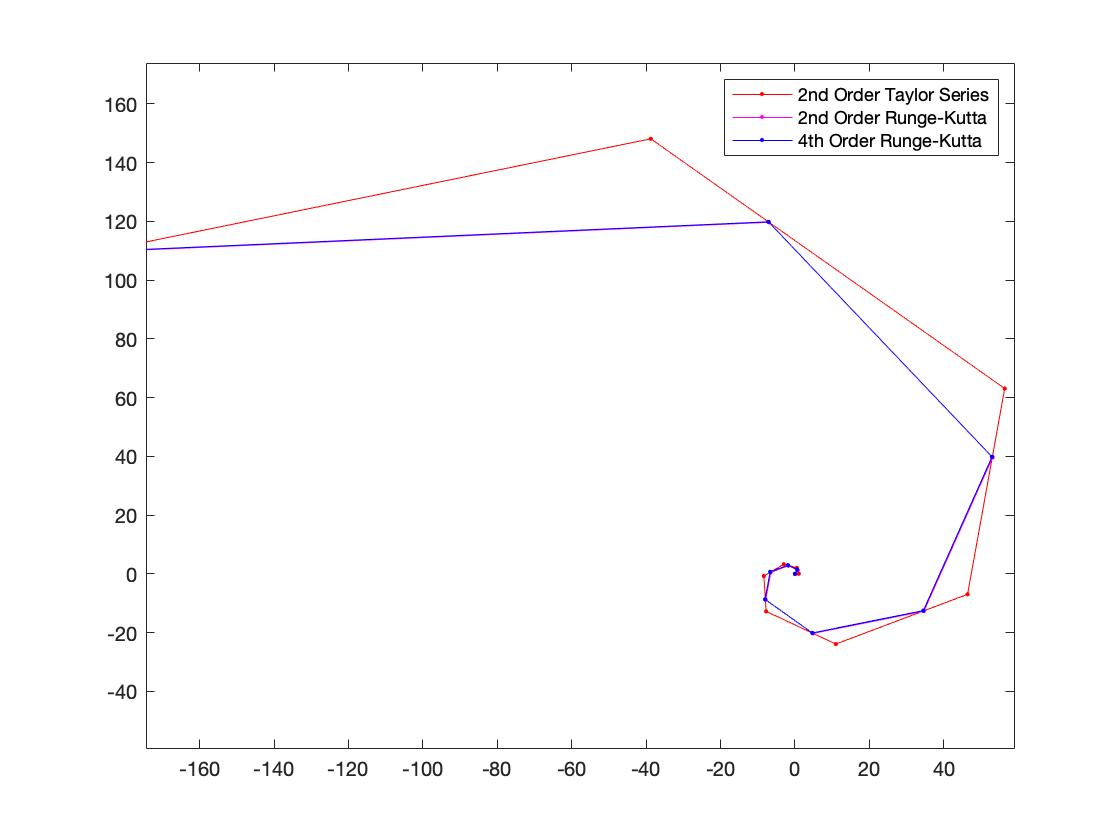
\includegraphics[width=\linewidth]{docs/h1.jpg}
  \caption{h = 1}
  % \label{fig:boat1}
\end{figure}

\begin{figure}[H]
  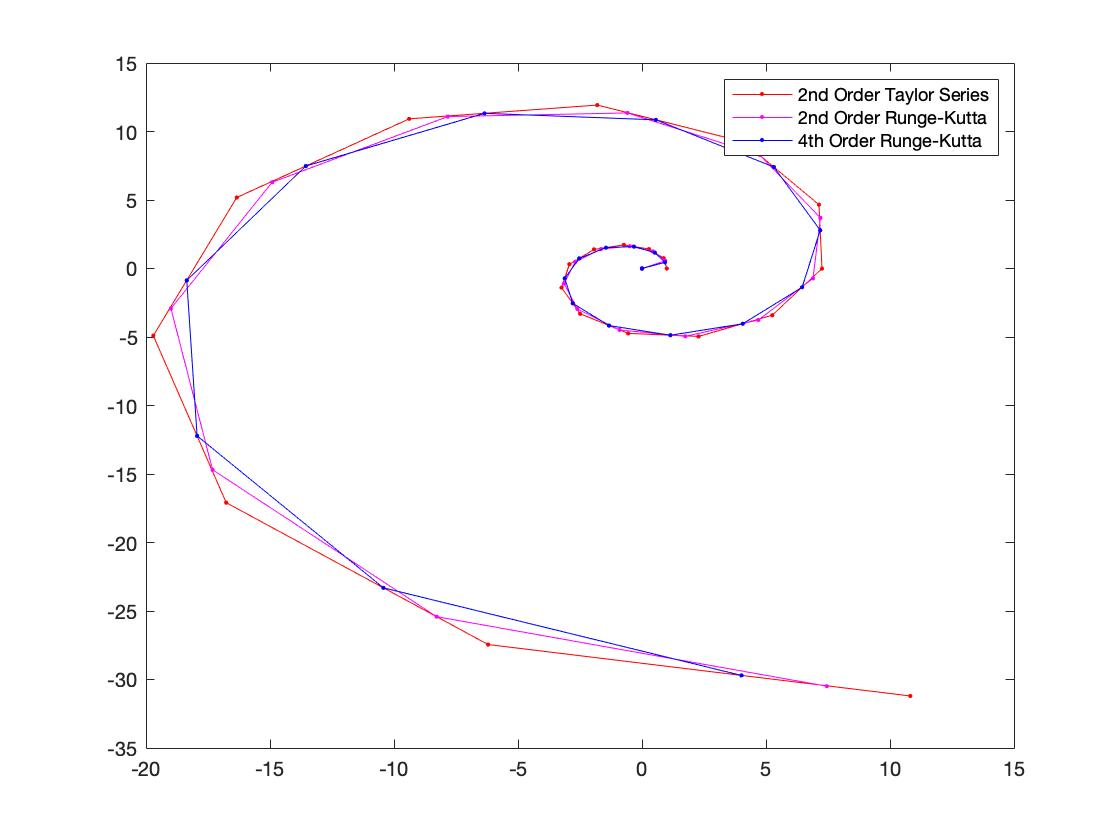
\includegraphics[width=\linewidth]{docs/05.jpg}
  \caption{h = 0.5}
\end{figure}

\begin{figure}[H]
  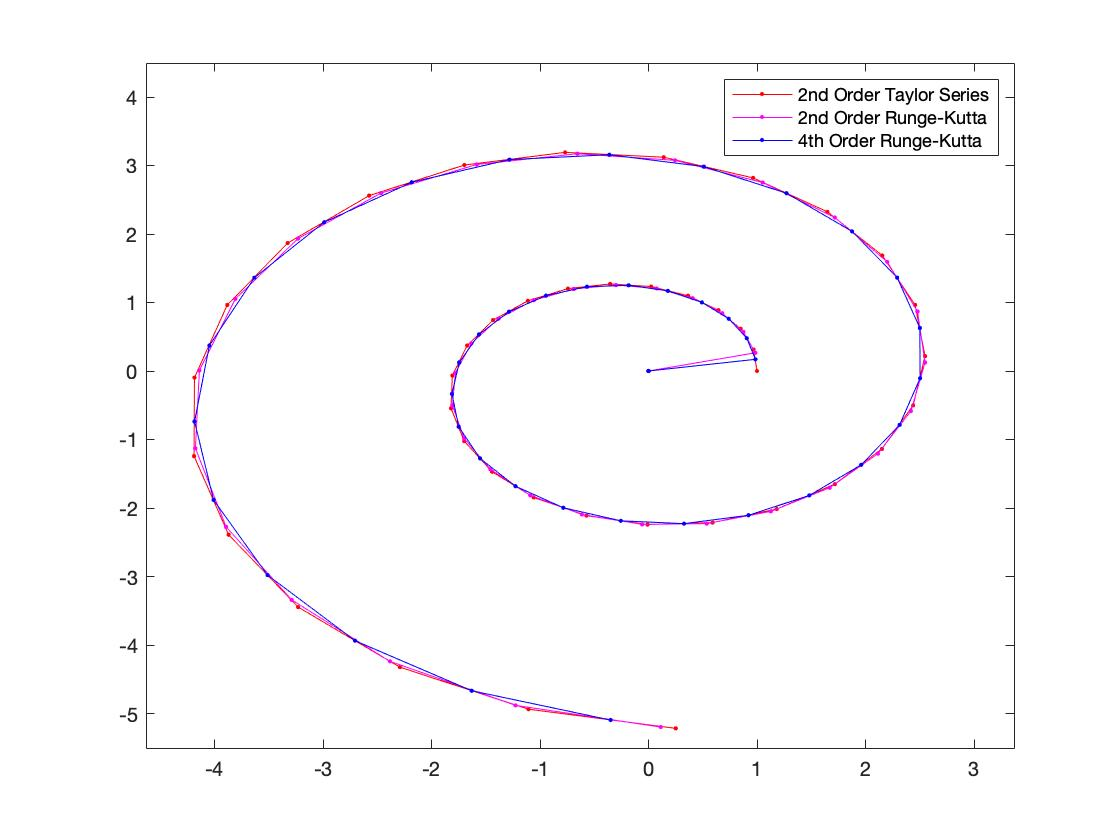
\includegraphics[width=\linewidth]{docs/h25.jpg}
  \caption{h = 0.25}
\end{figure}

\begin{figure}[H]
  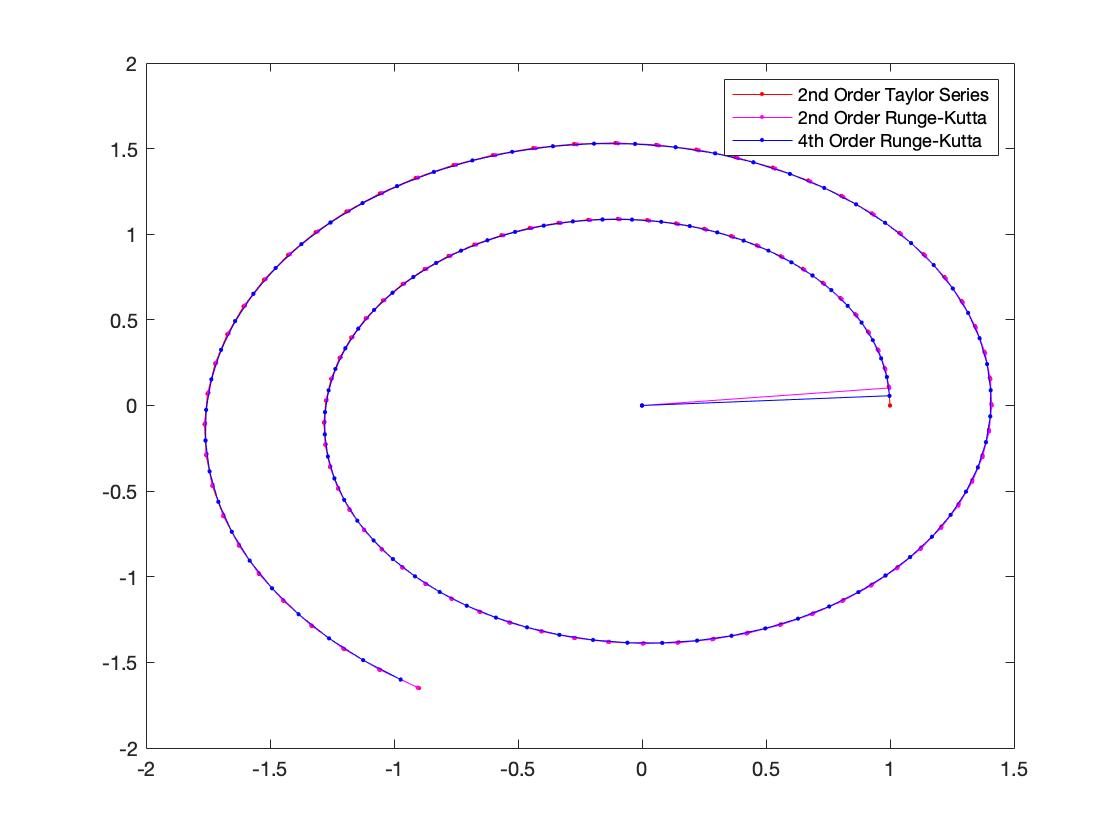
\includegraphics[width=\linewidth]{docs/0point1.jpg}
  \caption{h = 0.1}
\end{figure}


\section*{Problem 4}
Consider the following IVP

\begin{align*}
	x^{\prime} = x(1-x) \\
	x(0) = 0.01
\end{align*}
with the solution function $ x(t) = 1 - 1/(1 + e^{t}/99)$

\noindent
(a) Modify adaptive.m available on the course website to implement the Runge-Kutta-Fehlberg algorithm, provided below, to solve this IVP for $0 \leq t \leq 16$ The code should plot the analytical solution and the numerical solution on the same figure.

\lstinputlisting{/Users/allenspain/Documents/Development/MATLAB/comp-engr/hw6/RKF.m}

\begin{figure}[H]
  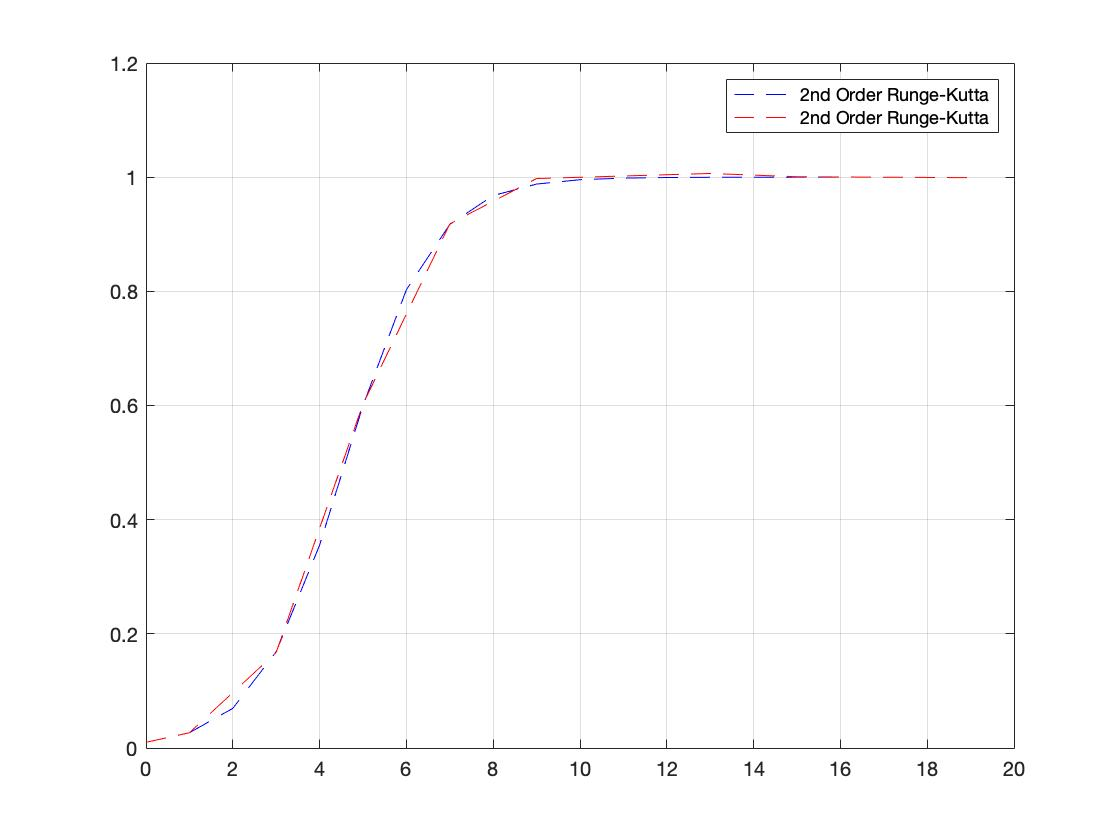
\includegraphics[width=\linewidth]{docs/01-rfk.jpg}
  \caption{tolerance = 0.01}
\end{figure}


\begin{figure}[H]
  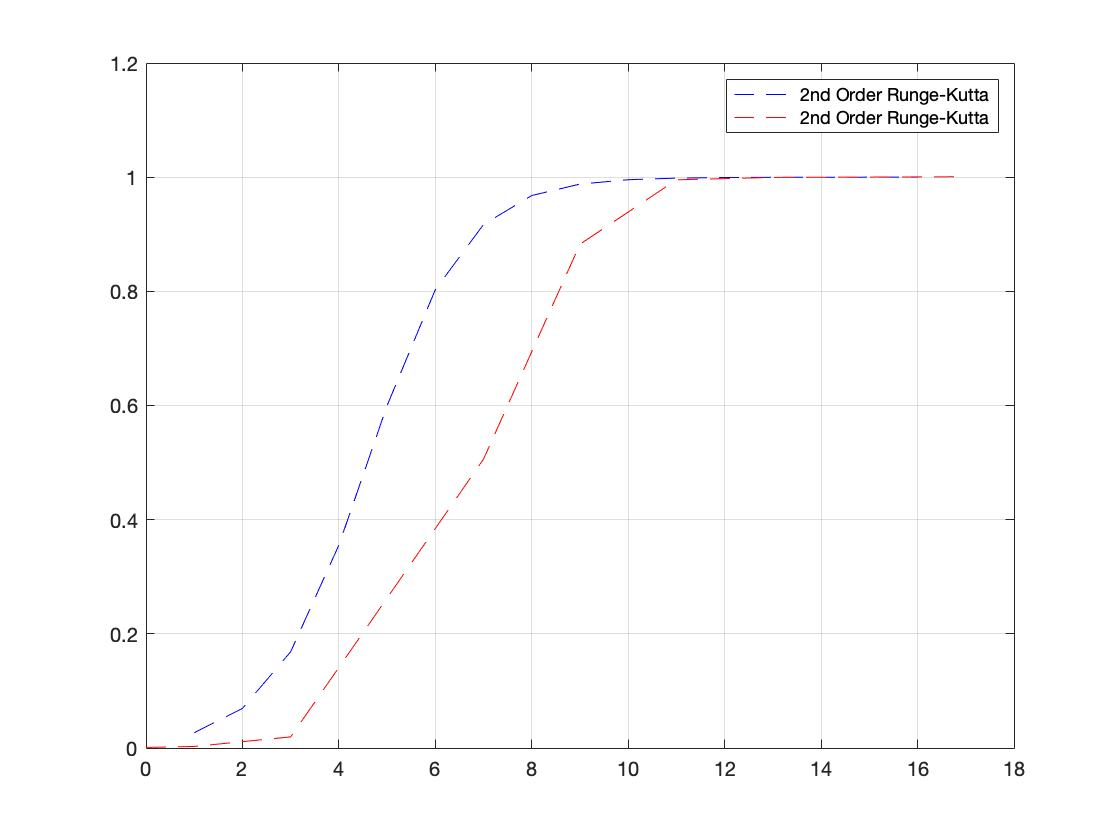
\includegraphics[width=\linewidth]{docs/001-rfk.jpg}
  \caption{tolerance = 0.001}
\end{figure}


=======
>>>>>>> 31adf8bead0ca3f0783d74f4a70004e23d603956
\end{document}
